%%%%%%%%%%%%%%%%%%%%%%%%%%%%%%%%%%%%%%%%%%%%%%%%%%%%%%%%%%%%%%%%%%%%%%%%%%%%%%%
% Chapter 'Adsorption - R-404a - activated carbon AquaSorb 2000'
%%%%%%%%%%%%%%%%%%%%%%%%%%%%%%%%%%%%%%%%%%%%%%%%%%%%%%%%%%%%%%%%%%%%%%%%%%%%%%%
\subsection{Activated carbon AquaSorb 2000}
%
%%%%%%%%%%%%%%%%%%%%%%%%%%%%%%%%%%%%%%%%%%%%%%%%%%%%%%%%%%%%%%%%%%%%%%%%%%%%%%%
%%%%%%%%%%%%%%%%%%%%%%%%%%%%%%%%%%%%%%%%%%%%%%%%%%%%%%%%%%%%%%%%%%%%%%%%%%%%%%%
\subsubsection{DubininAstakhov - ID 1}
%
\begin{tabular}[l]{|lp{11.5cm}|}
\hline
\addlinespace

\textbf{Sorbent:} & activated carbon \\
\textbf{Subtype:} & AquaSorb 2000 \\
\textbf{Refrigerant:} & R-404a \\
\textbf{Equation:} & DubininAstakhov \\
\textbf{ID:} & 1 \\
\textbf{Reference:} & Ghazy, Mohamed; Askalany, Ahmed A.; Harby, K.; Ahmed, Mahmoud S. (2016): Adsorption isotherms and kinetics of HFC-404A onto bituminous based granular activated carbon for storage and cooling applications. In: Applied Thermal Engineering 105, S. 639–645. DOI: 10.1016/j.applthermaleng.2016.03.057. \\
\textbf{Comment:} & See original literature: Use low-level interface for calculations as special form of density of adsorpt is required (i.e., rho\_adsorpt = A - B * T - rho\_gas(p, T) in kg/m3); inverse functions may not work anymore. \\

\addlinespace
\hline
\end{tabular}
\newline

\textbf{Properties of sorbent:}
\newline
%
\begin{longtable}[l]{lll}
\toprule
\addlinespace
\textbf{Property} & \textbf{Unit} & \textbf{Value} \\
\addlinespace
\midrule
\endhead
\bottomrule
\endfoot
\bottomrule
\endlastfoot
\addlinespace

Diameter of pore & \si{\milli\meter} & 0.00028\\
Surface area & \si{\square\meter\per\gram} & 1050\\
Pore volume & \si{\milli\cubic\meter\per\gram} & 1.04\\
Bulk density & \si{\kilogram\per\cubic\meter} & 480\\

\addlinespace\end{longtable}

\textbf{Equation and parameters:}
\newline
%
Loading $w$ in $\si{\kilogram\per\kilogram}$ is calculated depending on pressure $p$ in $\si{\pascal}$, temperature $T$ in $\si{\kelvin}$, and vapor pressure $p_\mathrm{sat}$ in $\si{\pascal}$ by:
%
\begin{equation*}
\begin{split}
w &=& \begin{cases} W \rho_\mathrm{sat}^{\mathrm{liq}} & \quad \text{if flag} \geq 0 \\ W & \quad \text{else} \end{cases} & \quad\text{, and} \\
W &=& W_0 \exp \left( - \left( \nicefrac{A}{E} \right) ^{n} \right) & \quad\text{, and} \\
A &=& R T \ln \left( \nicefrac{p_\mathrm{sat}}{p} \right) & \quad\text{.} \\
\end{split}
\end{equation*}
%
The parameters of the equation are:
%
\begin{longtable}[l]{lll|lll}
\toprule
\addlinespace
\textbf{Par.} & \textbf{Unit} & \textbf{Value} &	\textbf{Par.} & \textbf{Unit} & \textbf{Value} \\
\addlinespace
\midrule
\endhead

\bottomrule
\endfoot
\bottomrule
\endlastfoot
\addlinespace

flag & - & 1.000000000e+00 & $n$ & - & 1.030000000e+00 \\
$E$ & $\si{\joule\per\mole}$ & 9.578464000e+03 & $W_0$ & $\si{\cubic\meter\per\kilogram}$ & 1.035000000e-03 \\

\addlinespace\end{longtable}

\textbf{Validity:}
\newline
Equation is approximately valid for $14330.0 \si{\pascal} \leq p \leq 1179920.0 \si{\pascal}$,  $298.15 \si{\kelvin} \leq T \leq 348.15 \si{\kelvin}$, and $0.140971 \si{\kilogram\per\kilogram} \leq w \leq 0.519275 \si{\kilogram\per\kilogram}$.
\newline

\textbf{Visualization:}
%
\begin{figure}[!htp]
{\noindent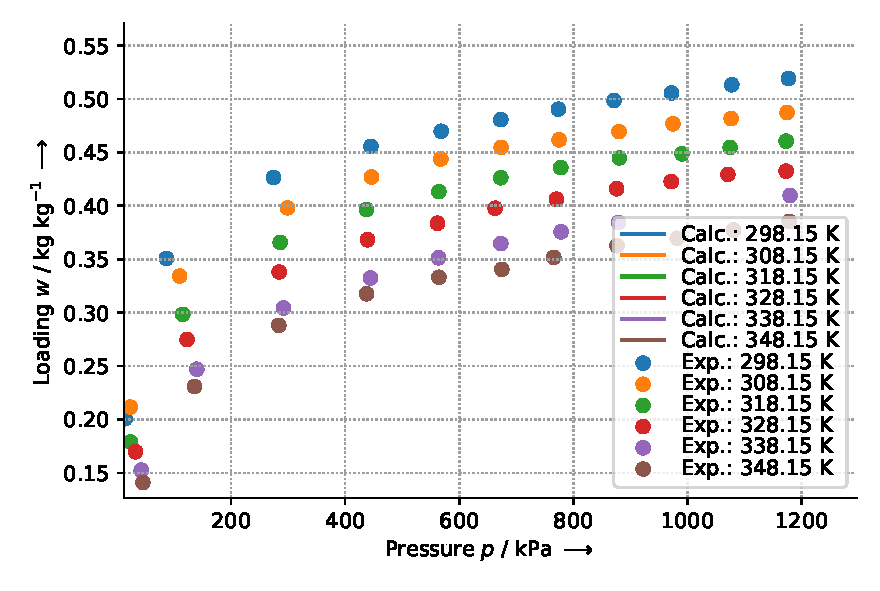
\includegraphics[height=10cm, keepaspectratio]{figs/ads/ads_R-404a_activated_carbon_AquaSorb_2000_DubininAstakhov_1.pdf}}
\end{figure}
%

To generate the figure, the following refrigerant functions were selected:
\begin{itemize}
\item Vapor pressure: NoVaporPressure - ID 1
\item Saturated liquid density: SaturatedLiquidDensity\_EoS1 - ID 1
\item Special refrigerant functions as described by comment and CoolProp
\end{itemize}

The uncertainity of the experimental data is:
\begin{itemize}
\item Data source $\,\to\,$ Data was taken from figure
\end{itemize}

The mean absolute percentage error (MAPE) between the experimental and calculated data results in 387.57\%.
\FloatBarrier
\newpage
%%%%%%%%%%%%%%%%%%%%%%%%%%%%%%%%%%%%%%%%%%%%%%%%%%%%%%%%%%%%%%%%%%%%%%%%%%%%%%%
